\scanpage{181}
\mspage{90}

of isomorphism of such a torsor is moreover identified, by the cohomology exact sequence \unsure{associated} with the exact sequence
\[
0 \longrightarrow \pi \longrightarrow
\pi\otimes_{\mathbb Z}\unsure{\mathbb C|\mathbb R}
\longrightarrow U_0 \longrightarrow 0
\]
\inserted{or \(\pi\otimes_{\mathbb Z}\mathbb R\)}
with a class of extensions of \(\Gamma\) by \(\pi\).
But to say that the action of \(\Gamma\) on \(\pi\) is trivial, means that the action of \(\Gamma\) on the torsor \(U\) under \(U_0\) is by translations.

\inserted{\uuline{Corollary-scholium}}
\uline{\unsure{N.B.}} The ``abelian'' case is not quite proved, for want of having established the \deleted{\unsure{topological}} classification \inserted{topological} of the operations of a finite group on \(\mathbb C^{*}\) or on \(S^1\times S^1\). However if in the abelian case we assume in advance that \(U^\Gamma\ne\varnothing\), \uline{then} \deleted{the conditions a) b) \unsure{c)}} it is still true that the trivial operation of \(\Gamma\) on \(\pi\) is equivalent to the triviality of the action of \(\Gamma\) on \(U\). For we are reduced to the case where \(\Gamma\) operates faithfully, and to proving in this case that if the operation of \(\Gamma\) on the \(\pi\) is trivial, we have \(\Gamma=1\). And we do as above in the anabelian case.

\scanpage{182}
\mspage{91}

\deleted{\unsure{Supplement|Deleted}}
\uline{18} \uline{Drilling holes.} Application to outer actions of finite groups

Let \(\Pi'\) be a group with loops of type \((g,\nu+1)\)\inserted{\(\unsure{(\nu+1\in\mathbb N^*)|(\nu\in\mathbb N^*)}\)}, nonabelian i.e. \deleted{\(g\ge2\) or \(g=1,\nu\ge1\) or} \inserted{\deleted{\illegible{1}}, \unsure{if}} \(g=0\), \inserted{\unsure{we have}} \(\nu\ge2\)
\deleted{(i.e. \(2g+\unsure{\nu\geq2}\quad 2g+\nu\ge\unsure{2|3}\) i.e. \(\deleted{\unsure{\geq}2}2-2g\,(=\mathrm{EP})\le\nu\)).}
Let \(T\) be its orientation module, and \(I'\) \((\operatorname{card}I'=\unsure{\nu})\) the set of its conjugacy classes of loop subgroups. Let us fix an \(i\in I'\), and let \(L'_i\subset\Pi'\) be in the class \(i\).

When we are given \deleted{\(\Pi'\) as} \inserted{only an} \uline{outer} group \deleted{\illegible{1}}\inserted{with loops \(\unsure{[\Pi']}\)} (which \deleted{\unsure{is done}} is equivalent to the datum of \(B_{D'^*}\longrightarrow B_{U'}\)), the datum of an \deleted{\illegible{1}} \(i\in I'\) is equivalent to that of a connected component of \(B_{D'^*}\), and that of a realization \deleted{\unsure{\((L_i,\Pi)\)}} of the categorical group (i.e. of a pair of a group \(\Pi'_{\unsure{s|\alpha}}\), and a categorical isomorphism \(\Pi'\longrightarrow[\Pi']_{\unsure{d}}\)) \inserted{is equivalent up to unique isomorphism} \deleted{\illegible{3}}\inserted{(universal covering \(\widetilde U'\) of \(U'\), by \(\Pi'=\operatorname{Aut}(\widetilde U')\).} of \(\Pi_1B_{U'}\), Finally the datum of a pair \((\Pi',L_i')\) (\(L_i'\) in the conjugacy class \(i\)) is equivalent \inserted{(up to unique isomorphism)} to the datum \unsure{of an} object \inserted{\(\widetilde D_i^{\unsure{*}}\)} of \(\Pi_1B_{D_i'^*}\) -- we take the image \(\widetilde U'\) of \(\widetilde D^{*'}\) in \(\Pi_1B_{U'}\), and
\[
\Pi'=\operatorname{Aut}(\widetilde U'),\qquad
L'_i=\operatorname{Im}\bigl(\operatorname{Aut}(\widetilde D_i'^*)\longrightarrow
\operatorname{Aut}(\widetilde U')\bigr).
\]
\margin{\unsure{I am going to} temporarily \unsure{drop} the ``primes''!}

When we are given \deleted{a realization} \inserted{\unsure{at the outset|whence a}} an object \(\widetilde U'_0\) of \(\Pi_1B_{U'}\), \unsure{whence} \inserted{\(\Pi'=\operatorname{Aut}(\widetilde U'_0)\)}, then

\scanpage{183}

the datum of an \(L_i\subset\pi\) in the class \(i\) is equivalent to the datum of a pair \((\widetilde D_i,\unsure{\lambda|\operatorname{id}})\) of a \(\widetilde D_i\in\operatorname{Ob}\Pi_1B_{D_i}\) and an isomorphism from \(\rho_!(\widetilde D_i)\unsure{=:|=}\widetilde U\) onto \(\widetilde U_0\).

When \deleted{\(\pi\) is realized} the topos-theoretic situation is realized from a topological situation \((X,S)\), and we define \(\widetilde U_0\) by means of a base point \(a\in U\), then the standard way of defining an \(L_i\subset\pi=\operatorname{Aut}(\widetilde U_0)=\pi_1(U,a)\) is to choose a small \unsure{disk} \(\Delta_i\) around \(s_i\) in \(X\),
\figure{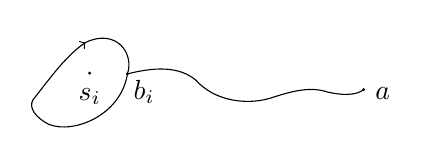
\begin{tikzpicture}[x=1cm,y=1cm,line cap=round,line join=round,baseline=(current bounding box.center)]
\coordinate (b) at (0.48,0.15);
\coordinate (a) at (3.48,-0.05);
\draw[->] (-0.72,-0.18) .. controls (-0.50,0.10) and (-0.30,0.38) .. (-0.05,0.55);
\draw (-0.05,0.55) .. controls (0.33,0.73) and (0.57,0.42) .. (b)
  .. controls (0.40,-0.37) and (-0.20,-0.62) .. (-0.52,-0.49)
  .. controls (-0.68,-0.41) and (-0.78,-0.28) .. (-0.72,-0.18);
\fill (0,0.16) circle (0.6pt);
\node[below] at (0,0.09) {$s_i$};
\fill (b) circle (0.6pt);
\node[below right,inner sep=2pt] at (b) {$b_i$};
\draw (b) .. controls (0.80,0.23) and (1.12,0.26) .. (1.35,0.07)
  .. controls (1.58,-0.19) and (1.98,-0.25) .. (2.29,-0.16)
  .. controls (2.59,-0.06) and (2.81,-0.01) .. (3.02,-0.08)
  .. controls (3.19,-0.12) and (3.38,-0.13) .. (a);
\fill (a) circle (0.6pt);
\node[right,inner sep=4pt] at (3.48,-0.10) {$a$};
\end{tikzpicture}}
and a point \inserted{\(b_i\)} on the boundary, and a homotopy class of paths \inserted{(in \(\deleted{\unsure{X}}\unsure{U|X}-(\mathring\Delta_i-\{s_i\})=V_i\))} from \(a\) to \(b_i\), and to take the group \(L_i\) generated by either one of the two corresponding loops around \(s_i\) (which give \deleted{\unsure{two}} opposite elements of \(\pi\)).
We see that we thus find a surjective map from
\[
\operatorname{Isom}_{\Pi_1V_i}(a,b_i)\simeq
\operatorname{Isom}_{\Pi_1U}(a,b_i)
\]
\deleted{to} onto the set of \(L_i\subset\pi\) in the class \(\unsure{i|\Pi}\), a map \deleted{whose} compatible with the

\scanpage{184}
\mspage{92}

natural action of \(\pi\) (operating on \(\operatorname{Isom}_{\Pi_1U}(a,b_i)\) in the obvious way by composition, and on the set of \(L_i\) by inner automorphisms.
\deleted{\unsure{Then}} Here, the \deleted{choice of} link with the ``abstract'' topos-theoretic description is established as follows: the choice of \(b_i\) can serve as a \unsure{base|fixed} point for defining a universal covering of \(\Delta_i\smallsetminus\{s_i\}\overset{\sim}{\hookleftarrow}D_i^*\), whence an object \(\rho_!(\widetilde D_i^*(b_i))\), and \deleted{\unsure{this object}} the \(L_i\subset\pi\) correspond \inserted{(according to the abstract description)} to the isomorphisms from \(\widetilde U_0=\widetilde U(a_i)\) onto \(\unsure{D_i^*(b_i)|\widetilde D_i^*(b_i)}\) modulo composition with an automorphism of \(\unsure{D_i^*(b_i)|\widetilde D_i^*(b_i)}\) coming from an automorphism of \(\unsure{D_i^*(b_i)|\widetilde D_i^*(b_i)}\) -- but the isomorphisms \deleted{from} \(\widetilde U(a_i)\xrightarrow{\sim}\rho_!(\widetilde D_i^*(b_i))\) correspond precisely to the classes of paths from \(a\) to \(b_i\).

\margin{We return to the notation \(\pi',U'\) --}
\unsure{Let us consider} an object of \(\Pi_1B_{D_i^{*'}}\), i.e. a pair \((\pi',L_i')\). Let \(\pi\) be the quotient group of \(\pi'\) by the invariant subgroup of \(\pi'\) \deleted{defined} \inserted{generated} by \(L_i'\). I say \margin{\(\Vert\)} that up to unique isomorphism (actual isomorphism of groups, not merely outer!) it does not

\scanpage{185}

depend on the choice of the object \(\widetilde D_i^*\) of \(\Pi_1B_{D_i'^*}\). Indeed, \(\pi=\pi(\widetilde D_i^*)\) depends functorially on \(\widetilde D_i^*\), and everything comes down to seeing that this functor is \uline{constant}, i.e. that the operation of
\[
\operatorname{Aut}(\widetilde D_i^*)\simeq T\simeq L_i
\quad\text{on}\quad
\pi=\pi(\widetilde D_i^*)
\]
is trivial. Now let \(u\in L_i\), \unsure{the|its} automorphism of \(\pi\) which it defines is defined by the inner automorphism \(\operatorname{int}(u)\) by passage to the quotient, hence (since \(u\) becomes \(1\) in \(\pi\)) it is trivial. \unsure{Easy.}

We thus find a \uline{functor}
\[
\begin{array}{c}
\text{Outer groups with loops }\pi'\\
\text{of type }g,\nu+1\text{ equipped with a}\\
\text{loop class }i\in I(\pi')
\end{array}
\longrightarrow
\begin{array}{c}
\text{groups}\\
\text{(realized)}\\
\text{with loops, of}\\
\text{type }g,\nu\deleted{\unsure{+1}}
\end{array}
\]
\[
(\pi',i)\longmapsto\beta(\pi',i)
\qquad
\text{[``plugging the hole \(i\)'']}
\]
which is expressed by a group homomorphism
\[
\operatorname{Aut\,ext}(\pi',i)\longrightarrow\operatorname{Aut}\pi
\tag{\unsure{*|5}}
\]
where \(\pi=\beta(\pi',i)\)
\[
\left(
\begin{array}{l}
\overset{\text{definition}}{=}\text{ set of categorical automorphisms}\\
\text{of }\pi'\text{ respecting the loop}\\
\text{structure and fixing the loop}\\
\text{class }i
\end{array}
\right)
\]

\scanpage{186}
\mspage{93}

From the geometric point of view, this fact (existence of this functor), merely expresses the fact that after ``plugging the hole'' \(i\), we have a \deleted{point} \(U=U'\cup\{s_i\}\) \uline{equipped} with a point \(s_i\) which we can use as a \uline{base point} \inserted{\uuline{canonical}} to calculate \(\pi_1(U)\).

We can also say that the choice of \(i\) makes it possible to construct the partial amalgamated sum (plugging holes \inserted{partially}) \(B_{U^*}\)
\diagram{
\begin{tikzcd}[ampersand replacement=\&]
\& B_{D_i'^*} \arrow[dl] \arrow[dr] \& \\
B_{U'} \arrow[dr] \& \& B_{s_i} \arrow[dl] \\
\& B_{U^*} \&
\end{tikzcd}
}
and \(B_{s_i}\longrightarrow B_{U^*}\) supplies a geometric point of \(B_{U^*}\) which makes it possible to describe a canonical object of \(\Pi_1B_{U^*}\) (universal covering relative to this point) whence canonically a group \(\pi\), which of course is a group with loops of type \(g,\nu-1\).

\uline{Theorem} Suppose \(g,\nu\) are such that not

\scanpage{187}

only the groups \(\pi'_{\unsure{s}}\) of type \(g,\nu\), but also the groups \(\pi\) (of type \(g,\nu-1\)) are anabelian, i.e.
\[
2g+\unsure{\nu}\deleted{\unsure{+1}}\unsure{\ge|\le}\unsure{4}
\quad
[\text{thus }g\ge2,\ \text{or }g\unsure{\ge|=}1,\nu\ge2,\ \text{or }g=0,\nu\ge4].
\]
Then the preceding functor \((\pi',i)\longrightarrow\pi\) is an equivalence of categories, in other words (since these are \(0\)-connected groupoids)
\[
\operatorname{Aut\,ext}(\pi',i)\longrightarrow\operatorname{Aut}(\pi)
\]
is an \uline{isomorphism}.

Let us note for this \unsure{that we have} the exact sequence
\[
1\longrightarrow\pi\longrightarrow\operatorname{Aut}(\pi)
\longrightarrow\operatorname{Aut\,ext}(\pi)\longrightarrow1:
\]
(for \(\operatorname{Centre}\pi=1\) by the anabelian hypothesis on \(\pi\)), \unsure{now} we are going to define an exact sequence
\[
1\longrightarrow\pi\longrightarrow\operatorname{Aut\,ext}(\pi',i)
\longrightarrow\unsure{\operatorname{Aut\,ext}(\pi)|\operatorname{Aut\,ext}(\pi')}
\longrightarrow1
\]
and a homomorphism of extensions from this one

\scanpage{188}
\mspage{\unsure{94|99}}

into the preceding one (which will necessarily be an isomorphism).

We may assume \(T=\mathbb Z\), we consider the \unsure{standard|standard} groups with loops \(\Pi_{g,\nu+1}\), \(\Pi_{g,\nu}\). Let us put
\[
\operatorname{Aut\,ext}_{\mathrm{lac}}(\Pi_{g,\nu})
=\unsure{\mathcal T|\mathfrak T}_{g,\nu}^{\unsure{00|\circ\circ}}
\]
\inserted{inducing \uline{the identity} on \(I(\Pi_{g,\nu})\) and on \(T(\Pi_{g,\nu})\)}
(Teichmüller group of index \(g,\nu\)),
we know that (for \(2g+\nu\ge3\)) \(\mathcal T_{g,\nu}\) is the fundamental group of the complex modular topos \inserted{\(M_{g,\nu}\)} of complex curves (\deleted{\illegible{1}} \unsure{projective nonsingular}) connected, of genus \(g\), with a system of \(\nu\) given distinct points \(s_1-\!s_\nu\).
\margin{\uline{N.B.} the universal covering of \(M_{g,\nu}\) is contractible, Teichmüller.}
Now the modular topos \(M_{g,\nu+1}\) is none other than \deleted{the image} the ``universal complex curve \deleted{\illegible{1}} of genus \(g\) with \(\nu\) numbered holes'' over \(M_{g,\nu}\)
[for giving ourselves a curve \inserted{\(U'\)} of genus \(g\) with \(\nu+1\) holes \inserted{\(x_1-\!x_{\nu+1}\)} amounts to the same as giving ourselves one \inserted{\(U\)} with \(\nu\) numbered holes \(x_1-\!x_\nu\), \uline{plus} a \deleted{hole of} point of \(U\) \deleted{\unsure{pointed}}), \uline{whence} a homotopy exact sequence
\diagram{
\begin{tikzcd}[ampersand replacement=\&,column sep=small]
\unsure{\pi_2|\Pi_2}(M_{g,\nu},\unsure{\xi})
 \arrow[r] \&
\pi_1(U) \arrow[r] \arrow[d,equal] \&
\pi_1(M_{g,\nu+1}) \arrow[r] \arrow[d,equal] \&
\pi_1(M_{g,\nu}) \arrow[r] \arrow[d,phantom,sloped,"\simeq"] \&
\pi_0(U) \arrow[d,equal] \\
0 \arrow[r] \&
\pi=\Pi_{g,\nu} \arrow[r] \&
\mathcal T^{00}_{g,\nu+1} \arrow[r] \&
\mathcal T^{00}_{g,\nu} \arrow[r] \&
1
\end{tikzcd}
}

\scanpage{189}

whence \unsure{an} extension structure \deleted{announced}
\[
1\longrightarrow\Pi_{g,\nu}
\longrightarrow\mathcal T^{00}_{g,\nu+1}
\longrightarrow\mathcal T^{00}_{g,\unsure{\nu}}
\longrightarrow1
\]
which is (up to passage to a subgroup of index ``\(2\nu!\)) this announced extension structure. \unsure{\&} the verifications of \uline{compatibility} are left \ldots.

We therefore have a quasi-inverse functor (defined up to unique isomorphism)
\[
\begin{array}{c}
\text{groups with loops}\\
\text{of type }g,\nu\\
(2g+\nu\ge3)
\end{array}
\longrightarrow
\begin{array}{c}
\text{\uline{outer} groups with}\\
\text{loops of type }(g,\nu+1),\\
\text{with a distinguished ``loop}\\
\text{class''}\\
\text{(pairs }(\pi',i\in I(\pi'))\text{)}
\end{array}
\]

\deleted{\unsure{Now}} \unsure{At the} topos-theoretic level, when we have a system \(B_{D^*}\longrightarrow B_U\) \inserted{of type \(g,\nu\) \((2g+\nu\ge3)\)}, and a ``point'' of \(B_U\) i.e. a \(\widetilde U\in\operatorname{Ob}\Pi_1B_U\), then we can in a canonical way find a \(B_{D_i^*}\) (\unsure{\(T\)-groupoid} \inserted{connected}, where \(T\) is the orientation module), and a system
\[
B_{D^*}\amalg B_{D_i^*}\longrightarrow B_{U'},
\]
of type \(g,\nu+1\),

\scanpage{190}
\mspage{95}

in such a way that \((B_{D^*},B_U,\widetilde U)\) \unsure{is deduced from it} by the operation of ``plugging the hole \(D_i^*\)''.

These constructions are so functorial, \margin{\unsure{\(\wedge\)}} that they commute with actions of groups \(\Gamma\). If a group \(\Gamma\) operates on a group with loops \(\pi_{\deleted{\unsure{g,\nu}}}\) of type \(g,\nu\), (not merely by outer automorphisms), then we deduce from it an \uline{outer} operation of \(\Gamma\) on a \(\pi'\) with loops of type \(g,\nu+1\), which fixes a privileged loop class \(i\in I\).

But then, in the corresponding extension
\[
1\longrightarrow\pi'\longrightarrow E'\longrightarrow\Gamma\longrightarrow1,
\]
Let us choose an \(L_i'\subset\pi'\) and let \(\unsure{\mathcal E_i'|E_i'}\) be the normalizer of \(L_i\) in \(\unsure{\mathcal E'|E'}\) -- we find
\[
1\longrightarrow
\underset{\simeq T}{L_i'}
\longrightarrow\unsure{\mathcal E_i'|E_i'}
\longrightarrow\Gamma\longrightarrow1
\]